\documentclass[output=paper
,modfonts
,nonflat]{langsci/langscibook} 

\title{Long distance agreement and information structure} 
\author{%
 Johannes Mursell\affiliation{Goethe-Universität Frankfurt am Main}
}
% \chapterDOI{} %will be filled in at production

% \epigram{}

\abstract{
In this paper, I discuss a specific subtype of long distance agreement (LDA), namely agreement across a finite (CP) clause boundary. I show that most, if not all, instances of LDA depend on information-structural properties of the agreement target in the embedded clause, be it for cross clausal object agreement or case assignment. After discussing LDA in unrelated language families, I argue that LDA is possible due to a complex probe in the left periphery containing information-structural features bundled with $ \phi $-features. This probe serves as an intermediate agreement step between a verb in the matrix clause and the information-structurally marked element in the embedded clause, so that LDA does not violate the phase impenetrability condition.
}

\begin{document}

\maketitle

\section{Introduction} 
Long distance agreement (LDA) in general refers to a syntactic dependency by which certain features, usually $ \phi $-features, of a probing head depend on features of a non-local constituent, i.e. a constituent not in the specifier of the probing head \citep{Bhatt_Keine2016}. While long distance agreement provides a strong argument for the operation of \textsc{agree} as formulated in \citet{Chomsky2000} and \citet{Chomsky2001}, and further refined in \citet{Pesetsky_Torrego2007}, which does not rely on local specifier-head agreement, several sub-cases of long distance agreement need to be distinguished.
\begin{exe} 
\ex \label{def:agr_pt} \textbf{Agree} \citep[][268]{Pesetsky_Torrego2007}
	\xlist
	\ex An unvalued feature F (a probe) on a head H at syntactic location $\alpha$ (F$_{\alpha}$) scans its c-command domain for another instance of F (a goal) at location $\beta$ (F$_{\beta}$) with which to agree. 
	\ex Replace F$_{\alpha}$ with F$_{\beta}$, so that the same feature is present in both locations.
	\endxlist
\end{exe}
The three cases of LDA that need to be distinguished differ from each other with respect to the distance between probe and goal. Those two elements can either be part of the same clause, separated by a non-finite clause boundary or by a finite one. The first case of LDA can be exemplified by quirky subjects in Icelandic or object agreement in Zulu. The example in (\ref{ex:ice}) from \citet{Zaenen_et_al1985} shows that in sentences with non-nominative subjects, a nominative object controls verbal agreement. Importantly, this nominative object is most likely not in the specifier of the projection that hosts \textit{voru} and thus, qualifies as a case of LDA.
\begin{exe} 
\ex Icelandic \citep[][460]{Zaenen_et_al1985}\label{ex:ice}\\ 
	\gll Konunginum voru gefnar amb\'{a}ttir.\\
	 the.king.\textsc{dat} were given.\textsc{f.pl} maidservants.\textsc{nom.f.pl}\\
	\glt `The king was given female slaves.'
\end{exe}
The second type, in which probing head and agreement target are separated by a non-finite clause boundary, can be found in English. In raising constructions, an expletive can be inserted in matrix subject position instead of raising the embedded subject. However, the embedded subject still controls agreement on the matrix verb.\footnote{Two reviewers point out that examples like (\ref{ex:engl_reg}) are possible in certain registers of English.}
\begin{exe}
\ex	
	\xlist
	\ex Two men seem to be in the garden.
	\ex There seem to be two men in the garden.
	\ex *There seems to be two men in the garden.\label{ex:engl_reg}
	\endxlist
\end{exe}
This type of cross-clausal long distance agreement, i.e. agreement into a non-finite clause, is present in several languages and has frequently been discussed in the literature. Thus, this type of agreement can be found in, among others, Hindi-Urdu \citep{Bhatt2005}, (\ref{ex:HU}), Godoberi \citep{Haspelmath1999}, (\ref{ex:God}), or Basque \citep{Preminger2009}.  
\begin{exe}
\ex
	\xlist
	\ex Hindi-Urdu \citep[][760]{Bhatt2005}\label{ex:HU}\\
		\gll Vivek-ne {[} \textbf{kitaab} pa\textipa{\r*r}h-nii] chaah-ii.\\
		 Vivek-\textsc{erg} {} \textbf{book.\textsc{f}} read-\textsc{inf.f} want-\textsc{pfv.\textbf{f}.sg}\\
		\glt `Vivek wanted to read the book.' \hfill 
	\ex	Godoberi  \citep[][136]{Haspelmath1999}\label{ex:God}\\
		\gll {[} wa\textipa{\u{s}}u-di \textbf{qu\textipa{\u{c}}i-be} r-al-u] \textbf{r}-uL-i.\\
		 {} boy-\textsc{erg} \textbf{book-\textsc{pl.abs}} \textsc{pl.n}-read-\textsc{cvb.pst} \textbf{\textsc{pl.n}}-finish-\textsc{aor}\\
		\glt `The boy finished reading the books.' \hfill
	\endxlist
\end{exe}
If long distance agreement into a non-finite clause is analysed as being based on a restructuring configuration \citep{Wurmbrand2001}, i.e. a configuration consisting of a full-fledged matrix clause and a truncated, smaller embedded clause, the two types of long distance agreement discussed so far do not challenge the locality of the agreement process in (\ref{def:agr_pt}), since neither violates the strong version of the Phase-Impenetrability Condition in (\ref{def:PIC}).
\begin{exe} 
	\ex \label{def:PIC} \textbf{Phase-Impenetrability Condition (PIC)} \citep{Chomsky2001}\\
	In a phase $ \alpha $ with head H, the domain of H is not accessible to operations outside $ \alpha $, only H and its edge are accessible to such operations.
\end{exe}
If phases are assumed to be at least CP and vP and if restructuring involves embedding clause smaller than CP, then agreement into a clause smaller than a CP does not violate the PIC.

The last and most surprising possibility of long distance agreement concerns instances in which probe and goal of the agreement process are separated by a finite CP boundary, and thus constitutes a clear violation of the PIC.\footnote{This presupposes that \textsc{agree} is subject to the same restrictions as movement. This is not undebated, see \citet{Boskovic2003,Boskovic2007}.} Examples for this type of LDA are rather rare but can be found in at least three different language families, namely in some of the Nakh-Dagestanian languages spoken in the north-eastern Caucasus region, in certain Algonquian languages spoken in north America, and in at least one Altaic language.

In those languages it is possible that, in certain circumstances, an argument of an embedded finite CP determines agreement on the matrix verb. In this paper, I will be concerned with the conditions in which this kind of long distance agreement can take place. I will argue that the crucial factor for LDA is that the embedded agreement goal is information-structurally marked, either as topic or as focus. This will also enable an analysis of the phenomenon compatible with PIC by agreement through the edge of the CP based on information-structural features, analyzing LDA as successive cyclic agreement comparable to successive cyclic wh-movement. In the discussion of LDA, an interesting generalization will emerge, namely that languages that allow LDA, allow it either for topics alone or for topics and foci, not however for foci alone.

\noindent The paper is structured as follows: I will first introduce the relevant phenomenon of LDA in more detail in Section \ref{ch:2} before I turn to previous analysis and their respective problems in Section \ref{ch:3}. In Section \ref{ch:4}, I develop my analysis and Section \ref{ch:5} concludes the paper.

\section{LDA crosslinguistically}
\label{ch:2}

Long distance agreement of the kind I am interested in in this paper is typologically much rarer than the other two types, but can be found in at least three different and unrelated language families. In this section, I am going to present the relevant data, pointing out the specific properties of the construction in the various languages based on the available literature, the properties any theory of LDA should be able to account for. First, the most well-known example, Tsez, will be presented, together with data from two other Nakh-Dagestanian languages, Hinuq and Khwarshi. Second, I will present data from the Algonquian languages Blackfoot, Innu-aim\^{u}n, and Passamaquoddy. In the last subsection, I will present data from an Altaic language, Uyghur, which displays a slightly different type of LDA, not based on $ \phi $-features but mostly on case.

As will become clear in this chapter, all languages share one important property: long distance agreement always takes place between an element of a higher phase and an information-structurally marked element of the lower phase. This information-structural marking will be at the heart of the analysis developed in section 4.

\subsection{Nakh-Dagestanian languages}

In their seminal paper, \citet{Polinsky_Potsdam2001} discuss LDA in the Nakh-Dagestanian language Tsez. The basic paradigm is given in (\ref{ex:lda_tsez}).
\begin{exe}
	\ex Tsez \citep[][584]{Polinsky_Potsdam2001} \label{ex:lda_tsez}
	\xlist
	\ex	\label{ex:tsez_top}
		\gll Eni-r [ u\textipa{\v{z}}\textipa{\=a} \textbf{magalu} b-\textipa{\=a}c’ru\textipa{\textbeltl}i ] \textbf{b}-iy-xo.\\
			 mother-\textsc{dat} [ boy \textbf{bread}.\textsc{\textbf{iii}.abs} ate ]	\textsc{\textbf{iii}}-know-\textsc{prs}\\
	 	\glt `The mother knows that, as for the bread, the boy ate it.' 
	\ex 
		\gll Eni-r [ u\textipa{\v{z}}\textipa{\=a} \textbf{magalu} b-\textipa{\=a}c’ru\textipa{\textbeltl}i ] \textbf{r}-iy-xo.\\
			 mother-\textsc{dat} [ boy \textbf{bread}.\textsc{\textbf{iii}.abs} ate ] \textsc{\textbf{iv}}-know-\textsc{prs}\\
	    \glt `The mother knows that the boy ate the bread.'
	\endxlist
\end{exe} 
In this ergative, verb-final language, only absolutive arguments determine agreement. As can be seen in (\ref{ex:tsez_top}), it is possible that the absolutive argument of the embedded clause determines noun class agreement on the matrix verb. As the translations of (\ref{ex:lda_tsez}) suggest, this is only possible if the embedded absolutive argument is interpreted as a topic; if it is not, the matrix verb shows default agreement (noun class \textsc{iv}). One possible solution to this problem would be to assume that `bread' in (\ref{ex:lda_tsez}) was actually scrambled into the matrix clause. However, as \citet[][590]{Polinsky_Potsdam2001} point out, Tsez does not show independent evidence for cross-clausal scrambling. Thus, the agreement pattern in (\ref{ex:lda_tsez}) constitutes an apparent violation of the PIC. The topic status of the agreement target can further be confirmed with overt topic marking, which is generally optional in Tsez. If the embedded absolutive is overtly topic marked, LDA becomes obligatory (\ref{ex:tsez_overt_top}). Furthermore, LDA is impossible with a focussed absolutive in the embedded clause (\ref{ex:tsez_overt_foc}).
\begin{exe}
	\ex Tsez \citep[][610-611]{Polinsky_Potsdam2001}
	\xlist
	\ex \label{ex:tsez_overt_top}
		\gll Eni-r [ u\textipa{\v{z}}\textipa{\=a} \textbf{magalu}-n/gon b-\textipa{\=a}c’ru\textipa{\textbeltl}i ] \textbf{b}/\textbf{*r}-iy-xo.\\
			mother-\textsc{dat} [ boy \textbf{bread}.\textsc{\textbf{iii}.abs-top} ate ] \textsc{\textbf{iii}}/\textsc{\textbf{iv}}-know-\textsc{prs}\\
		\glt `The mother knows that, as for the bread, the boy ate it.' 
	\ex \label{ex:tsez_overt_foc}
		\gll Eni-r [ \textbf{t'ek}-kin y-igu y\textipa{\=a\textbeltl}ru\textipa{\textbeltl}i ] \textbf{r/*y}-iy-xo.\\
			 mother-\textsc{dat} [ \textbf{book}.\textsc{ii.abs-foc}  \textsc{ii}-good be ] \textbf{\textsc{ii/iv}}-know-\textsc{prs}\\
	    \glt `The mother knows that the BOOK is good.'
	\endxlist
\end{exe}
The authors show that this agreement indeed crosses a clause boundary and that there is neither movement into the matrix clause nor a covert \textit{pro} co-referent with the embedded absolutive in the matrix clause. More important for the present purpose, there are further restrictions on long distance agreement in Tsez. Non-absolutive topics, either fronted or marked by a topic particle, block LDA.
\begin{exe}
	\ex Tsez \citep[][636]{Polinsky_Potsdam2001} \label{ex:tsez_nonabs_top}\\
		\gll Enir [ \textbf{\textipa{\textcrh}u\textipa{\textbeltl}} u\textipa{\v{z}}\textipa{\=a} magalu b\textipa{\=a}c’ru\textipa{\textbeltl}i ] \textbf{*b/r}-iy-xo.\\
		mother [ \textbf{yesterday} boy bread.\textsc{iii.abs} ate ] \textsc{\textbf{iii/iv}}-know-\textsc{prs}\\
		\glt `The mother knows that, yesterday, the boy ate it.'
\end{exe}
Non-absolutive wh-words, in-situ or ex-situ, also block LDA. Unfortunately, the absolutive wh-word \textit{\u{s}ebi} `who, what' shows class \textsc{iv} agreement which cannot be differentiated from agreement with the whole embedded clause/default agreement.
\begin{exe}
	\ex Tsez \citep[][634]{Polinsky_Potsdam2001} \label{ex:tsez_wh}\\
		\gll Enir [ \textbf{\textipa{\textbeltl}u} micxir b-ok'\textipa{\=a}kru\textipa{\textbeltl}i ] \textbf{*b/r}-iy-xo.\\
		 mother [ \textbf{who.\textsc{erg}} money.\textsc{iii.abs} \textsc{iii}-stole ]	\textsc{\textbf{iii/iv}}-know-\textsc{prs}\\
		\glt `The mother knows who stole the money.'
\end{exe}
D-linked wh-words in Tsez belong to different classes and can consequently be used to test the availability of LDA with wh-elements. And indeed, d-linked wh-elements can trigger long distance agreement .
\begin{exe}
	\ex Tsez \citep[][fn. 20]{Polinsky_Potsdam2001} \label{ex:tsez_wh_dlinked}\\
		\gll Enir [ \textbf{\u{s}ebi} y-\textipa{\=a}k'iru-\textipa{\textbeltl}i ] \textbf{y}-iy-x-\={a}nu.\\
			 mother [ \textbf{wh.\textsc{ii.abs}} \textsc{ii}-went-C ] \textbf{\textsc{ii}}-know-\textsc{prs-neg}\\
		\glt `The mother does not know who [of women] left.'
\end{exe}
Lastly, LDA is also blocked by the presence of the overt complementizer \textit{-ƛin} (\ref{ex:tsez_comp_block}). In contrast, the complementizer \textit{-\textipa{\textbeltl}i} does not block LDA, as can be seen from the previous examples.
\begin{exe}
	\ex Tsez \citep[][635]{Polinsky_Potsdam2001}\label{ex:tsez_comp_block}\\
		\gll *Enir [ u\textipa{\v{z}}\textipa{\=a} \textbf{magalu} b-\textipa{\=a}c’-si-\textbf{ƛin} ] \textbf{b}-iy-xo.\\
			 mother [ boy \textbf{bread.\textsc{\textbf{iii}.abs}} \textsc{\textbf{iii}}-eat-\textsc{pst.evid}-\textsc{\textbf{c}} ]	\textsc{\textbf{iii}}-know-\textsc{prs}\\
		\glt int.: `The mother knows that, as for the bread, the boy ate it.'
\end{exe}
The fact that the two complementizers behave differently is puzzling at first glance. \citet[][fn 19]{Polinsky_Potsdam2001} suggest that \textit{\textipa{\textbeltl}i} should not be treated as a complementizer at all but rather as a derivational suffix. A different possibility would be to assume that the two complementizers occupy different positions in a complex left periphery, as has been proposed for Italian \citep{Ledgeway2005}. For the analysis to be presented in section \ref{ch:4}, it is only important to note that at least one type of complementizer blocks LDA.

Long distance agreement in the Nakh-Dagestanian languages is not just restricted to Tsez but also present in at least two other related languages, namely Khwarshi and Hinuq.\footnote{See \textcitetv{chapters/10-boerjesson-mueller} for a discussion of LDA in Nakh-Dagestanian languages.}

In Khwarshi \citep{Khalilova2008,Khalilova2009} long distance agreement is possible into complement clauses of verbs of cognition,\footnote{The other mentions that LDA possible into complement clauses of verbs of cognition but only gives examples for \textit{to know} and also does not provide a reason for this behavior. From the author's discussion of the examples, it might be concluded that the reason for this is related to case: the subject of \textit{to know} surfaces in lative case and the other argument with absolutive which enables the other argument to determine agreement.} and, in contrast to Tsez, embedded topics and embedded foci can be targeted. Again, only absolutive arguments show agreement and in addition to LDA with the embedded absolutive, the matrix verb can also show class \textsc{iv} agreement, which can either be treated as agreement with the whole complement clause or as default agreement, comparable to Tsez. In (\ref{ex:kwarshi}), an example for LDA with an embedded topic is shown. In its in-situ position, the topic can cause optional LDA with the matrix verb. If the topic is fronted to the matrix clause, however, then the matrix verb obligatory agrees with the fronted topic.
\begin{exe}
\ex Khwarshi  \citep[][118]{Khalilova2008}\label{ex:kwarshi}
	\xlist
	\ex
		\gll U\v{z}a-l \textbf{b/l}-iq'-\v{s}e [ \textbf{zihe-n} b-iti-xx-u].\\
			 boy.\textsc{obl-lat}  \textbf{\textsc{iii/iv}}-know-\textsc{prs} {} \textbf{cow}(\textbf{\textsc{iii}})-\& \textsc{iii}-divide-\textsc{caus}-\textsc{pfv.cvb}\\
		\glt `The boy knows that the cow was stolen.'
	\ex
		\gll \textbf{Zihe-n} u\v{z}a-l \textbf{b}-iq'-\v{s}e [ b-iti-xx-u].\\
			 \textbf{cow}(\textbf{\textsc{iii}})-\& boy.\textsc{obl-lat} \textbf{\textsc{iii}}-know-\textsc{prs} {} \textsc{iii}-divide-\textsc{caus}-\textsc{pfv.cvb}\\
		\glt `The boy knows that the cow was stolen.'
	\endxlist
\end{exe}
In addition to embedded topics, embedded foci, more specifically answers to d-linked wh-questions, can also show long distance agreement. In d-linked wh-questions, the pattern is similar to (\ref{ex:kwarshi}): the wh-element in the embedded clause can determine agreement on the matrix verb, while agreement with the whole complement clause remains a possible but dispreferred option. 
\begin{exe}
\ex Khwarshi  \citep[][390]{Khalilova2008}\\
	\gll [ dogu \textbf{zihe} b-ot'uq'q-u ] \textbf{b/l}-iq'-\v{s}e u\v{z}a-l?\\
		 {} which \textbf{cow}(\textbf{\textsc{iii}}) \textsc{iii}-come-\textsc{pst.ptcp} {} \textbf{\textsc{iii/iv}}-know-\textsc{prs} boy.\textsc{obl-lat}\\
	\glt `Which cow does the boy know came?'
\end{exe}
Similarly in the answer, the LDA pattern is preferred over the local agreement. If the constituent corresponding to the wh-element in the question is fronted, then LDA becomes obligatory. Since constituents that correspond to wh-elements in the respective questions usually carry focus, I assume that not only topic but also focus on the agreement goal can license LDA in Khwarshi.
\begin{exe}
\ex Khwarshi  \citep[][390]{Khalilova2008}
	\xlist
	\ex
		\gll u\v{z}a-l \textbf{b/l}-iq'-\v{s}e [ \textipa{k\super Q}aba \textbf{zihe} b-ot'uq'q-u ].\\
			 boy.\textsc{obl-lat} \textbf{\textsc{iii/iv}}-know-\textsc{prs} {} black \textbf{cow}(\textbf{\textsc{iii}}) \textsc{iii}-come-\textsc{pst.ptcp} {}\\
		\glt `The boy knows that the black cow has come.'
	\ex
		\gll [ \textipa{k\super Q}aba \textbf{zihe} b-ot'uq'q-u ] \textbf{b}-iq'-\v{s}e u\v{z}a-l.\\
			 {} black \textbf{cow}(\textbf{\textsc{iii}}) \textsc{iii}-come-\textsc{pst.ptcp} {} \textbf{\textsc{iii}}-know-\textsc{prs} boy.\textsc{obl-lat}\\
		\glt `The boy knows that the black cow has come.'	
	\endxlist
\end{exe}
Those complement clauses that allow LDA in Khwarshi are formed based on a nominalized form of the embedded verb, compatible with a clause union / restructuring analysis (\citealt{Haspelmath1999} for Godoberi). However, \citet[386-388]{Khalilova2009} explicitly argues for a bi-clausal analysis based on the behaviour of reflexives and adverbs as well as the scope of negation. Thus, Khwarshi constitutes another language in which cross-clausal long distance agreement is possible, differing from Tsez in the fact that not only topics but also foci can participate in LDA.

The last Nakh-Dagestanian language to be discussed is Hinuq \citep{Forker2012}. Again, only absolutive arguments agree and in cases in which LDA is possible, the verb can either show noun class agreement with the embedded absolutive or agreement with the whole complement clause/default agreement, which is class \textsc{v}. While the class of matrix verbs that allow LDA is bigger than in Khwarshi, the status of the agreement target is similar, it can either be a topic (\ref{ex:hinqu_top}) or a focus (\ref{ex:hinqu_foc}).
\begin{exe}
\ex Hinuq \citep[][628]{Forker2012}
	\xlist
	\ex \label{ex:hinqu_top}
		\gll Hay\textipa{\textbeltl}o-z \textbf{b}-ike-s [ \textbf{me\v{s}i} \v{c}eq-i-do b-i\textipa{L}'i-\v{s} ].\\
			 he.\textsc{obl}-\textsc{dat} \textbf{\textsc{iii}}-see-\textsc{pst} {} \textbf{calf}(\textbf{\textsc{iii}}) forest-\textsc{in}-\textsc{dir} \textsc{iii}-go-\textsc{pst}\\
		\glt `He saw that the calf went into the forest.' 
	\ex  \label{ex:hinqu_foc}
		\gll Pat'imat-ez \textbf{y}-eq'i-yo [ Madina-y \textbf{t'ek} y-ux-i\u{s}-\textipa{\textbeltl} ].\\
			 Patimat-\textsc{dat} \textbf{\textsc{iv}}-know-\textsc{prs} {} Madina-\textsc{erg} \textbf{book(\textsc{iv})} \textsc{iv}-buy-\textsc{res-abst}\\
		\glt `Patimat know that Madina bought the BOOK.'
	\endxlist
\end{exe}
In contrast to Tsez, non-absolutive wh-elements do not block LDA, and absolutive wh-elements can themselves be agreement targets in LDA constructions.
\begin{exe}
\ex Hinuq \citep[][637]{Forker2012}
	\xlist
	\ex
		\gll \u{S}amil-ez \textbf{r/b}-eq'i-yo [ ni Madina-y \textbf{mecxer} b-uqi-\u{s}-\textipa{\textbeltl}i ].\\
			 Shamil-\textsc{dat} \textbf{\textsc{v/iii}}-know-\textsc{prs} {} where Madina-\textsc{erg} \textbf{money(\textsc{iii})} \textsc{iii}-hide-\textsc{res-abst}\\
		\glt `Shamil knows where Madina hid the money.'
	\ex 
		\gll Obu-z \textbf{r/\O{}}-eq'i-yo [ ked-ez \textbf{\textipa{\textbeltl}u} \O{}-ike-s-\textipa{\textbeltl}i ].\\
			 father-\textsc{dat} \textbf{\textsc{v/i}}-know-\textsc{prs} {} girl-\textsc{dat} \textbf{who(\textsc{i})} \textsc{i}-see-\textsc{res-abst}\\
		\glt `Father knows who the girl saw.'
	\endxlist
\end{exe}
Another interesting difference concerning LDA in Hinuq is that it is possible across several clauses. In a sentence with three clauses, LDA is easily possible when the higher verbs all show non-local agreement (\ref{ex:hinuq_non-loc}). It is also possible that only the intermediate verb(s) show non-local agreement (\ref{ex:hinuq_med}), but non-local agreement of the highest verb and local agreement of the intermediate one is dispreferred (\ref{ex:hinuq_high}).
\begin{exe}
\ex Hinuq \citep[][633]{Forker2012} \label{ex:hinuq_cross-clausal}
	\xlist
	\ex \label{ex:hinuq_non-loc}
		\gll ʡali-\v{z} \textbf{b}-eti-yo [ [ obu-y ec'endiyu \textbf{ma\v{s}ina} b-ux-\textipa{L}'os-\textipa{\textbeltl}i ] Madina-z \textbf{b}-eq'-ayaz ].\\
			 Ali-\textsc{dat} \textbf{\textsc{iii}}-want-\textsc{prs} {} {} father-\textsc{erg} new \textbf{car}(\textbf{\textsc{iii}}) \textsc{iii}-buy-\textsc{hab}-\textsc{abst} {} Madina-\textsc{dat} \textbf{\textsc{iii}}-know-\textsc{purp}\\
		\glt `Ali wants Madina to know that father will buy a new car.'
	\ex \label{ex:hinuq_med}
		\gll Murad-ez \textbf{r}-eq'i-yo [ \textipa{\textcrh}akim-ez \textbf{y}-eti-n [ de \textbf{ka\textipa{G}at} cax-a ] ].\\
			 Murad-\textsc{dat} \textbf{\textsc{v}}-know-\textsc{prs} {} ruler-\textsc{dat} \textbf{\textsc{iv}}-want-\textsc{uwpst} {} I.\textsc{erg} \textbf{letter}(\textbf{\textsc{iv}}) write-\textsc{inf}\\
		\glt `Murad knows that the boss wants me to write a letter.'
	\ex \label{ex:hinuq_high}
		\gll ?di-\v{z} \textbf{b}-eti-n [ debez \textbf{r}-eq'-a [ \textipa{\textbeltl}u-y \textbf{gulu} b-ik'ek-i\v{s}-\textipa{\textbeltl}i ] ].\\
			 I-\textsc{dat} \textbf{\textsc{iii}}-want-\textsc{uwpst} {} you.\textsc{sg.dat} \textbf{\textsc{v}}-know-\textsc{inf} {} who-\textsc{erg} \textbf{horse}(\textbf{\textsc{iii}}) \textsc{iii}-steal-\textsc{res}-\textsc{abst}\\
		\glt `I want you to know who stole the horse.'
	\endxlist
\end{exe}
Thus, even though all three languages presented in this section allow LDA, the exact implementation varies. The most important point of variation concerns the status of the agreement target, the DP in the embedded clause. While in Tsez it is only possible when the embedded DP is interpreted as a topic, Hinuq and Khwarshi allow LDA with embedded foci as well. In the next section it will be shown that the same type of variation can be found in the Algonquian language family.

\subsection{Algonquian languages}

A second language family in which some languages show LDA are the Algonquian languages spoken in North America over a large area, stretching from the east coast through to the Rocky Mountains. The patterns of LDA found in this language family are remarkably similar to LDA in Nakh-Dagestanian languages, in that a precondition for LDA is that the agreed-with DP in the embedded clause receives a special information-structural interpretation.\footnote{See \citet{Fry_Hamilton2014} for a comprehensive discussion of LDA in Algonquian languages.}

Starting with Innu-aim\^{u}n, as discussed in \citet{Branigan_MacKenzie2002}, a very similar pattern to Tsez emerges. Certain matrix verbs take complement clauses and can show agreement either with the $ \phi $-features of the embedded subject (\ref{ex:innu_decl_subj}), (\ref{ex:innu_q_subj}), or the embedded object (\ref{ex:innu_decl_obj}), (\ref{ex:innu_q_obj}). However, LDA is always optional, and agreement with the whole complement clause/default agreement is possible (\ref{ex:innu_default}), which in Innu-aim\^{u}n is similar to transitive inanimate (TI) agreement, the agreement with inanimate objects. The complement clause is fully specified for tense and can be declarative (\ref{ex:innu_decl}) or interrogative (\ref{ex:innu_int}), thus strongly suggesting a CP-sized complement clause.\footnote{Agreement in Innu-aim\^{u}n and Passamaquoddy is very complex and a full discussion beyond the scope of the paper. I have marked the relevant agreement marker and the argument it references in bold. For further details about the agreement systems and details on the glossing, the reader is referred to the referenced literature.} %The proofreader complains about certain points in the glosses, and rightly so, because they don't seem to fit the example. However, I double-checked, and that is the way they have it in the cited source.
\begin{exe}
\ex Innu-aim\^{u}n \citep[][388]{Branigan_MacKenzie2002} \label{ex:innu_decl}
	\xlist
	\ex \label{ex:innu_default}
		\gll Ni-tshissenitamu-\^{a}n\^{a}n [ m\^{u}pishtu\^{a}t Sh\^{u}shepa Tsh\^{a}n m\^{a}k Ma\^{a}n\^{i} ].\\
			 \textsc{1pl}-know-\textsc{\textbf{ti}-1pl} {} visit Joseph John and Marie\\
		\glt `We know that John and Marie visited Joseph.'
	\ex \label{ex:innu_decl_subj}
		\gll Ni-tshissenim-\^{a}n\^{a}n-\textbf{at} [ m\^{u}pishtu\^{a}t Sh\^{u}shepa \textbf{Tsh\^{a}n} \textbf{m\^{a}k} \textbf{M\^{a}n\^{i}} ].\\
			 \textsc{1pl}-know-\textsc{1pl-\textbf{3pl}} {} visit Joseph \textbf{John} \textbf{and} \textbf{Marie}\\
		\glt `We know that John and Marie visited Joseph.'
	\ex \label{ex:innu_decl_obj}
		\gll Ni-tshissenim-\^{a}n\^{a}n [ m\^{u}pishtu\^{a}t \textbf{Sh\^{u}shepa} Tsh\^{a}n m\^{a}k M\^{a}n\^{i} ].\\
			 \textsc{1pl}-know-\textsc{1pl-\textbf{3sg}} {} visit \textbf{Joseph} John and Marie\\
		\glt `We know that John and Marie visited Joseph.'
	\endxlist
\end{exe}
\begin{exe}
\ex Innu-aim\^{u}n \citep[][399]{Branigan_MacKenzie2002} \label{ex:innu_int}
	\xlist
	\ex	\label{ex:innu_q_subj}
		\gll Ma tshi-tshissenim-\textbf{in} [ {t\^{a}n ishpish na} \textbf{nit}-aim\^{a} M\^{a}n\^{i} ]?\\
			 \textsc{q} \textsc{2sg}-know-\textbf{\textsc{1sg}} {} when \textbf{\textsc{1sg}}-called Marie\\
		\glt `Do you know when I called Marie?'
	\ex \label{ex:innu_q_obj}
		\gll Ma tshi-tshissenim-\textbf{\^{a}u} [ {t\^{a}n ishpish na} nit-aim\^{a} \textbf{M\^{a}n\^{i}} ]?\\
			 \textsc{q} \textsc{2sg}-know-\textbf{\textsc{3sg}} {} when \textsc{1sg}-called \textbf{Marie}\\
		\glt `Do you know when I called Marie?'
	\endxlist
\end{exe}
Since Innu-aim\^{u}n is a pro-drop language, the agreement target in LDA frequently is a dropped pronoun. Interestingly, if LDA takes place, the agreed-with DP can be moved to the front of the embedded clause. This movement is impossible if LDA is absent. Similar to Passamaquoddy discussed below, the question arises whether the moved embedded DP ends up in a position in the matrix clause or a left-peripheral position of the embedded clause. The authors, in contrast to \citet{Bruening2001a} for Passamaquoddy, assume that the DP ends up in the matrix clause. However, (\ref{ex:innu_disloc}) is also compatible with the dislocated DP still being in the embedded clause, simply higher than the wh-element or complementizer. %Do I pick this up later? I.e. when explicit topicalization in the embedded clause, LDA becomes obligatory?
\begin{exe}
\ex Innu-aim\^{u}n \citep[][389]{Branigan_MacKenzie2002} \label{ex:innu_disloc}
	\xlist
	\ex	
		\gll Tshi-tshissenim-\textbf{\^{a}u}-\^{a} [ \textbf{M\^{a}n\^{i}} tsheku\^{a}n {kuet aimi\^{a}t} P\^{u}na utshim\^{a}minua ]?\\
			 \textsc{2sg}-know-\textsc{ta}-\textbf{\textsc{3sg}}-\textsc{q} {} \textbf{Marie} why called Paul boss\\
		\glt `Do you know why Marie called Paul's boss?'
	\ex \label{ex:innu_q}
		\gll N-u\^{i}-tshissenim-\textbf{\^{a}u} [ kassinu \textbf{k\^{a}u\^{a}pikueshit} tshetsh\^{i} m\^{u}pisht\^{a}shkuenit ].\\
			 \textsc{1sg}-want-know-\textbf{\textsc{3sg}} {} every \textbf{priest} if visited-\textsc{2sg}/\textsc{inv}\\
		\glt `I want to know if every priest visited you.'
	\endxlist
\end{exe}
The authors argue at length against a proxy-agreement account, to be discussed shortly, and instead propose that the agreement target in the embedded clause carries an unvalued A'-feature that they term \textit{O}-feature which allows it to move covertly into the specifier of the CP so it is available for agreement with the matrix verb. Additionally, the authors claim that the agreement goal in the embedded clause is usually interpreted as the topic of that clause, so that the most likely candidate for the \textit{O}-feature is a topic feature. This is in line with the observation mentioned earlier that the LDA goal is frequently a dropped pronoun, a highly topical element. The only qualification to this assumption is presented by wh-elements, since they also can appear as targets for LDA. Thus, the left periphery seems to play the crucial role in licensing LDA: either the LDA agreement goal is information-structurally marked or moved high enough in the left periphery of the embedded clause due to independent reasons like wh-movement.\footnote{Unfortunately, the authors do not discuss whether the wh-element can be targeted for LDA when a topicalised element precedes it.}

Thus, Innu-aim\^{u}n shows many properties of LDA already discussed for Nakh-Dagestanian languages, since it is possible either with embedded topics or with wh-elements in the left periphery of the embedded clause. Similarly, if the embedded agreed-with DP is overtly topic marked by dislocation, LDA is obligatory, just as in Tsez when the topic is marked overtly by a particle.

Another Algonquian language that shows long distance agreement is Passamaquoddy \citep{Bruening2001a}. Here, the picture is more complex, just as the data in Hinuq appear to be more complex than in Tsez. Passamaquoddy has a raising to object construction, raising the embedded object across embedded C, that causes object agreement on the matrix verb (\ref{ex:passam_rto}). However, the actual raising part of this operation is optional, such that a LDA configuration is created (\ref{ex:passam_lda}), in which the matrix verb does not need to agree with the highest argument in the embedded clause. If LDA takes place, the agreed-with argument in the lower clause is usually interpreted as topical or focussed.
\begin{exe}
\ex Passamaquoddy \citep[][258]{Bruening2001a}\label{ex:passam_rto}
	\xlist
	\ex	
		\gll '-Kosiciy-a-\textbf{l} [ yaq \textbf{uhsimis-ol} eli keka peciya-li-t ].\\
			 \textsc{3sg}-know.\textsc{ta-dir-\textbf{obv}} {} \textsc{quot} \textbf{3.younger.sib-\textsc{obv}} \textsc{c} almost come-\textsc{obv.s-3sg.conj}\\
		\glt `She knew that her brother had almost arrived.'
	\ex 
		\gll Susehp '-kosiciy-\textbf{\`{a}} [ \textbf{ak\`{o}m} eli Muwin kisi-mil-at Wiphun].\\
			 Susehp \textsc{3sg}-know.\textsc{ta-dir.\textbf{obv.pl}} {} \textbf{snowshoe.\textsc{obv.pl}} \textsc{c} M. \textsc{perf}-give-\textsc{3sg.conj} W.\\
		\glt `Susehp knows that Muwin gave Wiphun snowshoes.'
	\endxlist
\end{exe}
\begin{exe}
\ex Passamaquoddy \citep[][259]{Bruening2001a}\label{ex:passam_lda}
	\xlist
	\ex	\label{ex:passam_ti_lda}
		\gll N-wewitaham-a-\textbf{k} [ ma=te nomiy-a-w-ik \textbf{mawsuwinuw-ok} Kehlis-k ].\\
			 \textsc{1sg}-remember-\textsc{dir-\textbf{3pl}} {} \textsc{neg=emph} see-\textsc{dir-neg-part.3pl} \textbf{person-\textsc{3pl}} Calais-\textsc{loc} {}\\
		\glt `I remember that I didn't see people in Calais.'
	\ex
		\gll N-kosicihtun-ol [ eli Piyel nokkaht-aq \textbf{sukolis-ol} wikahtm-an-pon-il ].\\
			 \textsc{lsg}-know.\textsc{ti-\textbf{inan.pl}} {} \textsc{c} Piyel eat.up-\textsc{3sg.conj} \textbf{candy-\textsc{inan.pl}} like.eat-\textsc{l.conj-pret-part.inan.pl}\\
		\glt `I know that Piyel ate up the candies that I liked.'
	\endxlist
\end{exe}
LDA is also possible in embedded questions, either with the wh-element (\ref{ex:passam_wh}) or a different argument. If LDA in embedded questions takes place with an argument different from the wh-element and is also accompanied by overt movement, this agreed-with argument may end up in a position to the left of the embedded wh-element  (\ref{ex:passam_wh_arg_front}). Since Passamaquoddy is a wh-movement language, the fronted argument consequently either occupies a position in the left periphery even higher than the wh-element in the embedded clause or a low position already in the matrix clause, similar to what \citet{Branigan_MacKenzie2002} argue for Innu-aim\^{u}n. The author argues extensively for the first option, which thus makes LDA in Passamaquoddy similar to LDA in the Nakh-Dagestanian languages.
\begin{exe}
\ex Passamaquoddy \citep[][259]{Bruening2001a}
	\xlist
	\ex \label{ex:passam_wh}	
		\gll Tihtiyas ma=te wewitaham-a-wiy-\textbf{il} [ \textbf{wen-il} amsqahs kis-aqosom-uw-iht kiwhosu ].\\
			 Tihtiyas \textsc{neg=emph} remember-\textsc{dir-neg-\textbf{obv}} {} \textbf{who-\textsc{obv}} first \textsc{perf}-cook-\textsc{appl-3sg.conj.inv} muskrat.\textsc{obv.pl}\\
		\glt `Tihtiyas doesn't remember who first cooked muskrat for her.'
%	\ex \label{ex:passam_wh_arg}
%		\gll N-kosiciy-a-k keq nuhuw-ok muwinuw-ok kis-temu-htit.\\
%			 1-know.\textsc{ta-dir-3.p} what three-\textsc{3.p} bear-\textsc{3.p} \textsc{perf-}eat\textsc{-3.p.conj}\\
%		\glt `I know what the three bears ate.'
	\ex \label{ex:passam_wh_arg_front}
		\gll N-kosiciy-a-\textbf{k} [ \textbf{nuhuw-ok} muwinuw-ok keq  kis-temu-htit ].\\
			 \textsc{1sg}-know.\textsc{ta-dir-\textbf{3pl}} {} \textbf{three-\textsc{3pl}} \textbf{bear-\textsc{3pl}} what \textsc{perf-}eat\textsc{-3pl.conj}\\
		\glt `I know what the three bears ate.' 
	\endxlist
\end{exe}
Similarly to \citet{Branigan_MacKenzie2002} for Innu-aim\^{u}n, \citet{Bruening2001a} conclusively argues against possible alternatives to the movement analysis. However, the exact nature of the landing site of the movement in the left periphery of the embedded clause is not clear. The agreement target in the embedded clause is compatible with either a topic or a focus interpretation. This is shown by either marking the embedded argument with the contrastive topic marker \textit{olu}, (\ref{ex:passam_topmark}), or modifying it with the focus sensitive particle \textit{tehpu} `only', (\ref{ex:passam_focmark}).
\begin{exe}
\ex Passamaquoddy \citep[][282]{Bruening2001a}
	\xlist
	\ex \label{ex:passam_topmark}
		\gll Ma=te n-kosiciy-\textbf{a}-wi [ \textbf{wot} \textbf{olu} \textbf{n-tatat}, tan-iyut keti-nomkuwal-s-it atomupil ].\\
			 \textsc{neg} \textsc{1sg}-know.\textsc{ta-dir-neg} {} \textbf{this.\textsc{an}} \textbf{\textsc{top}} \textbf{\textsc{1sg}-father} \textsc{wh}-this.\textsc{inan} \textsc{ic.fut}-lend-\textsc{intrans-3sg.conj} car\\
		\glt `I don't know which car, my father, he's going to buy.'
	\ex \label{ex:passam_focmark}
		\gll N-kosiciy-\textbf{a} [ \textbf{tehpu} \textbf{Susehp} oc menuwa-c-ihi nuhu akom ].\\
			 \textsc{1sg}-know.\textsc{ta-\textbf{dir}} {} \textbf{only} \textbf{Susehp} \textsc{fut} \textsc{ic}.buy-\textsc{3sg.conj-part.obv.pl} three.\textsc{obv.pl} snowshoe.\textsc{obv.pl}\\
		\glt `I know that only Susehp would buy three snowshoes.'
	\endxlist
\end{exe}
If two possible agreement targets compete, i.e. when the embedded clause contains a focus and a topic, the topic can be the target of LDA while skipping the focussed argument, as already shown in \ref{ex:passam_wh_arg_front}, where a topic serves as goal for LDA despite the presence of a focussed element, the wh-word.

This leads \citet{Bruening2001a} to the conclusion that the landing position of the raising to object movement cannot be a single dedicated topic or focus projection. Assuming a split-CP analysis \citep{Rizzi1997}, the data are compatible with an analysis of the landing position in terms of discourse projections: both the topic projection and the focus projection can serve as a landing site for raising to object movement and agree with the respective constituent. \footnote{Some data appear to be incompatible with this analysis. Singular, non-referential quantifiers can appear in embedded questions preceding wh-elements (\ref{ex:passam_qr}).
\begin{exe}
\ex {\normalfont Passamaquoddy \citep[][282]{Bruening2001a}}\label{ex:passam_qr}\\ %no idea if NORMALFONT works here
	\gll Sapet '-kosiciy-a-\textbf{l} [ \textbf{psi=te} \textbf{wen-il} tan-iyuhtol nucitqonkelic-il kisi-tqon-at ].\\
		 Sapet \textsc{3sg}-know.\textsc{ta-dir-obv} {} \textbf{all=\textsc{emph}} \textbf{someone-\textsc{obv}}  \textsc{wh}-that.\textsc{obv} policeman-\textsc{obv} \textsc{perf}-arrest-\textsc{3sg.conj}\\
	\glt `Sapet knows which policeman arrested everybody.'
\end{exe}
However, first, it is not obvious that the fronted quantifiers cause long distance agreement on the matrix verb. If the language provides other means to move an element in the embedded clause above the wh-element, then LDA could for example also be based on overt QR. Second, \citet{Bruening2001a} argues that sometimes the element that appears to have undergone raising to object is actually initially merged in the matrix clause, which could also be the case for (\ref{ex:passam_qr}). Thus the data do not constitute counterevidence to the information-structural dependence of LDA.} These data show striking similarities with respect to LDA not only between Passamaquoddy and Innu-aim\^{u}n, but also between those two languages from the Algonquian family and the languages from the Nakh-Dagestanian family, Tsez, Khwarshi, and Hinuq.

As already pointed out by \citet{Polinsky2003}, it is important when discussing LDA in Algonquian languages to carefully distinguish genuine LDA from cases of proxy-agreement or prothetic agreement which is not a case of LDA even though it appears to be one on the surface. In those languages that are viable to that kind of analysis, a silent pronoun in the matrix clause, which is co-referential with the element in the embedded clause serves as the actual agreement target of the matrix predicate.\footnote{At least one argument used by \citet{Polinsky2003} in favor of a proxy-agreement account is directly addressed and dismissed by \citet{Bruening2001a} as well as \citet{Branigan_MacKenzie2002}. In Passamaquoddy as well as Innu-aim\^{u}n, agreement on the matrix verb can be with a subset of the goal in LDA configurations. Polinsky argues this is due to a \textit{pro} in the matrix clause, but \citet[][269]{Bruening2001a} shows that it can also occur in contexts which definitely involve movement like relative clauses and thus dismisses this argument.} Due to the co-referentiality of the proxy argument in the matrix clause and the embedded argument, such a structure appears to show LDA even though only clause bound agreement is involved. Such a construction would be similar to English (\ref{ex:ENG_proxy}), with the matrix pronoun being a silent \textit{pro}.
\begin{exe}
\ex *Peter knows of her that Mary went to the movies. \label{ex:ENG_proxy}
\end{exe}
Note the ungrammaticality of (\ref{ex:ENG_proxy}), which is due to a violation of Principle C. Even though Principle C is not necessarily active in all Algonquian languages, \citet{Branigan_MacKenzie2002} argue that it does play a role in Innu-aim\^{u}n and thus an analysis along the lines of proxy agreement is not feasible. This is supported by further arguments, for example the impossibility of having an English (\ref{ex:ENG_pro}) with a proxy argument in the matrix clause, i.e. having a prothetic pronoun co-referring with a wh-element.
\begin{exe}
\ex *Do you know of him who is laughing? \label{ex:ENG_pro}
\end{exe}
For Passamaquoddy, \citet{Bruening2001a} also discusses and dismisses a proxy agreement account, relying on the same arguments as \citet{Branigan_MacKenzie2002}. He shows that having an overt pronoun in the matrix clause doubling the embedded DP is ungrammatical, probably due to a Principle C violation, (\ref{ex:passam_pro}). The observation that LDA in Passamaquoddy can also target the wh-element of the embedded clause and that embedded wh-elements cannot be coreferential with a matrix pronoun (cf. \ref{ex:ENG_pro}), provides another argument against a proxy agreement analysis.\footnote{The author also argues against a different kind of the proxy agreement analysis in which either a proxy or the full DP is base generated in the left periphery of the embedded clause, comparable to a left dislocation construction. I cannot discuss this here for reasons of space, but  \citet[][263ff]{Bruening2001a} provides ample evidence that movement inside the embedded clause does indeed take place.}
\begin{exe}
\ex Passamaquoddy \citep[][270]{Bruening2001a} \label{ex:passam_pro}
	\xlist
	\ex 
		\gll N-kosiciy-\textbf{a} [ eli \textbf{Piyel} koti-nathula-t Susehp-ol ].\\
			 \textsc{1sg}-know.\textsc{ta}-\textbf{\textsc{dir}} {} \textsc{c} \textbf{Piyel} \textsc{fut}-pick.up.in.boat-\textsc{3sg.conj} Susehp-\textsc{obv}\\
		\glt `I know that Piyel will pick up Susehp in a boat.'
	\ex
	 	\gll *N-kosiciy-\textbf{a} \textbf{nekom} [ eli \textbf{Piyel} koti-nathula-t Susehp-ol ].\\
			 \textsc{1sg}-know.\textsc{ta}-\textsc{dir} \textsc{3sg} {} \textsc{c} Piyel \textsc{fut}-pick.up.in.boat-3\textsc{sg.conj} Susehp-\textsc{obv}\\
		\glt `I know about him that Piyel will pick up Susehp in a boat.'
	\endxlist
\end{exe}
Before closing this section, it should be pointed out that even though the proxy-agreement account of LDA cannot be applied to LDA in Passamaquoddy or Innu-aim\^{u}n, other Algonquian languages do seem to present cases of agreement by proxy. Blackfoot for example does show apparent LDA (\ref{ex:black_lda}). Blackfoot also presents an apparent counterexample to the generalization stated in the beginning that either topic and focus can serve as LDA targets in a given language or topic alone, since \citet{Bliss2009} argues that LDA in Blackfoot marks contrastive foci.
\begin{exe}
\ex Blackfoot \citep[][1]{Bliss2009}\label{ex:black_lda}\\
	\gll nit-iksstaat-a an-wa Leo nin-aahk-sspommo-a-hsi.\\
		 \textsc{1sg}-want.\textsc{ta}-\textsc{1sg:3sg} \textsc{dem-prox} Leo 1-\textsc{mod}-help.\textsc{ta-1sg:3sg-conj}\\
	\glt `I want to help Leo.'
\end{exe}
However, LDA in Blackfoot has been analysed as proxy agreement and thus does not constitute a proper case of LDA and therefore also not a counterexample to the generalization stated above. \citet{Polinsky2003}, going back to \citet{Frantz1978}, discusses several phenomena that can be linked to LDA by proxy. One of them concerns binding. In Blackfoot, since the proxy in the matrix clause constitutes a full pronoun, it can actually bind a reflexive on the verb.
\begin{exe}
\ex Blackfoot \citep[][99, via Polinsky 2003: 286]{Frantz1978}\\
	\gll noxk\'{o}wa ki niist\'{o}wa nits-\'{i}ksstat-tsiiyi-xpinnaani n-\'{a}xk-a'po'tak-ss-innaan.\\
		 my.son.3 and \textsc{1sg} \textsc{1sg}-want-\textsc{recp}-1\textsc{pl} 1-might-work-\textsc{conj-1pl}\\
	\glt lit.: `My son and I want of each other that we work.'
\end{exe}
I have argued in this section, that in addition to languages in the Nakh-Da\-ges\-ta\-nian family, some Algonquian languages also show LDA, also conditioned by information-structural properties of the embedded agreement target. Similarly to Nakh-Dagestanian languages, two types of LDA targets can be distinguished in Algonquian languages: either agreement with both topics and foci is possible, as in Passamaquoddy, or LDA is restricted to topics as in Innu-aim\^{u}n. Additionally, I have also distinguished LDA proper from LDA by proxy, as exemplified by Blackfoot. Concerning LDA by proxy in Nakh-Dagestanian languages, \citet{Polinsky2003} has argued that Tsez show proper LDA. This has not been discussed explicitly for Hinuq or Khwarshi, but data strongly suggest an analysis in the line of Tsez. The next subsection will discuss LDA in yet another unrelated language family, however in a slightly different context.

\subsection{LDA in Uyghur}

Another, less frequently discussed, case of an apparent PIC violating dependency is exceptional subject case marking in Altaic languages. In many languages from this family, subjects in certain types of finite embedded clauses can occur with a case other than nominative, mostly genitive but also accusative. Even though the occurrence of non-canonical subject case is different from the LDA agreement pattern discussed above, in which a matrix verb agrees with an argument in a complement clause, those cases could still constitute instances of LDA, namely when the exceptional case is licensed from outside the clause and the clause itself is of CP size. Thus, these two aspects need to be considered carefully, and Table \ref{tab:exc_s_c} shows that, as expected, significant variation along these two dimensions can be found in the Altaic languages.
\begin{table}
\caption{Exceptional Subject Case in Altaic.}
\label{tab:exc_s_c}
 \begin{tabular}{lll} 
  \lsptoprule
  Language  & Emb. clause size & Licenser for subject\\
  \midrule
  Turkish \citep{Kornfilt2008} & CP & clause internal C\\
  Dagur \citep{Hale2002} & AspP ($ < $CP) & clause external D\\
  Japanese \citep{Miyagawa2011} & TP ($ < $CP) & clause external D\\
  Uyghur \citep{Asarina_Hartman2011a} & CP & clause external D\\
  \lspbottomrule
 \end{tabular}
\end{table}

As can be seen in the table, Uyghur seems to present the right configuration that exceptional subject case could be analyzed as LDA, since the case of the subject in a CP is licensed by an element from outside that CP. If case licensing is taken to be based on agreement, and this analysis is correct, then Uyghur shows a case of LDA. Examples of this configuration are given in (\ref{ex:uyg_lda}).
\begin{exe}
\ex Uyghur \citep[][4]{Asarina_Hartman2011b}\label{ex:uyg_lda}
	\xlist
	\ex 
		\gll [ \textbf{Men-\textipa{1N}} ji-gen ] tamaq-\textbf{im} ja\textipa{XS}i.\\
		 	 {} \textbf{\textsc{1sg}-\textsc{gen}} eat-\textsc{ran} {} food-\textbf{1\textsc{sg.poss}} good\\
		\glt `The food that I ate is good.'\label{ex:uyg_1sg}
	\ex
		\gll [ \textbf{Ötkür-n\textipa{1N}} oqu-\textipa{K}an ] kitav-\textbf{i} uzum.\\
			 {} \textbf{Ötkür-\textsc{gen}} read-\textsc{ran} {} book-\textbf{3\textsc{sg.poss}} long\\
		\glt `The book that Ötkür read is long.'\label{ex:uyg_3sg}
	\ex
		\gll [ Ötkür oqu-\textipa{K}an ] kitap uzum.\\
			 {} Ötkür read-\textsc{ran} {} book long\\
		\glt `The book that Ötkür read is long.'\label{ex:uyg_no}
	\endxlist
\end{exe}
In order to make this point more clear, I will summarize the discussion in \citet{Asarina_Hartman2011a}, first showing that it is indeed clause external D that licenses genitive subject case in relative clauses and NP complement clauses in Uyghur and second, also presenting arguments in favour of a CP sized embedded clause. The first argument for licensing \textsc{gen} on the embedded subject by an external head comes from agreement with the embedded subject that shows up on the external D head only when the subject carries genitive case, (\ref{ex:uyg_1sg}-\ref{ex:uyg_3sg}). If the embedded subject is unmarked (which is a free variant), then there is no agreement on the external D (\ref{ex:uyg_no}). The second piece of evidence comes from the observation that clause external D can only assign genitive once. Thus the sentence in (\ref{ex:uyg_amb}) is ambiguous, and double genitives as in (\ref{ex:uyg_dgen}) are impossible.
\begin{exe}
\ex Uyghur \citep[][3]{Asarina_Hartman2011a}
	\xlist
	\ex \label{ex:uyg_amb}
		\gll Ajgül-nu\textipa{N} resim-i\\
			 Aygül-\textsc{gen} picture-3\textsc{sg.poss}\\
		\glt `picture belonging to Aygül' or `picture depicting Aygül'
	\ex \label{ex:uyg_dgen}
		\gll *Ötkür-n\textipa{1N} Ajgül-nu\textipa{N} resim-i\\
			 Ötkür-\textsc{gen} Aygül-\textsc{gen} picture-3\textsc{sg.poss}\\
		\glt int.: `picture that depicts Aygül and belongs to Ötkür'
	\endxlist
\end{exe}
If in relative clauses and nominal complements the clause external D head is responsible for genitive assignment to the subject of the embedded clause, genitive subjects should be in complementary distribution with genitive possessors while unmarked subjects should be able to occur with genitive possessors since the genitive of the clause external D is still available when it is not assigned to the subject. The data in (\ref{ex:uyg_gen_ass}) show that this prediction is borne out.
\begin{exe}
\ex Uyghur \citep[][3]{Asarina_Hartman2011a} \label{ex:uyg_gen_ass}
	\xlist
	\ex 
		\gll *[ Ötkür-n\textipa{1N} oqu-\textipa{K}an] Ajgül-nu\textipa{N} kitav-i uzum.\\
			 {} Ötkür-\textsc{gen} read-\textsc{ran} Aygül-\textsc{gen} book-3\textsc{sg.poss} long\\
		\glt int.: `Aygül's book that Ötkür read is long.'
	\ex
		\gll [ Ötkür oqu-\textipa{K}an] Ajgül-nu\textipa{N} kitav-i uzum.\\
			 {} Ötkür read-\textsc{ran} Aygül-\textsc{gen} book-3\textsc{sg.poss} long\\
		\glt `Aygül's book that Ötkür read is long.'
	\endxlist
\end{exe}
Following the authors, I conclude from this that the genitive subject is indeed licensed from outside the clause. However, to analyze this phenomenon as a case of LDA proper, it is also necessary to show that the embedded clauses are CPs and not smaller constituents as in other Altaic languages. The authors support the assumption of CP sized embedded clauses with two arguments, CP adverbs and embedded questions. First, if the embedded clause can host CP adverbs, then it must be treated as a CP. The clause initial adverb \textit{\textipa{X}eqiqi} `truly' in (\ref{ex:uyg_advs}) shows the possibility of CP adverbs.
\begin{exe}
\ex Uyghur \citep[][8]{Asarina_Hartman2011a}\label{ex:uyg_advs}
	\xlist
	\ex 
		\gll [ \textipa{X}eqiqi \textbf{Ajgül-ni\textipa{N}} jaz-\textipa{K}an ]  kitiv-\textbf{i}-ni korset!\\
			 {} truly \textbf{Aygül-\textsc{gen}} write-\textsc{ran} {} book-\textsc{3sg.poss}-\textsc{acc} show\\
		\glt `Show me the book that Aygül truly wrote.'
	\ex
		\gll [ \textipa{X}eqiqi m\textbf{en-i\textipa{N}} ja\textipa{XS}i kör-i-gen ] tamaq-\textbf{im}-ni ber!\\
			 {} truly \textbf{I-\textsc{gen}} well see-\textsc{impf}-\textsc{ran} {} food-\textbf{\textsc{1sg.poss}}-\textsc{acc} give\\
		\glt `Give (me) the food that I truly like.'
	\endxlist
\end{exe}
Second, the embedded clause can also be a question and it is argued that interpretation as a question necessarily requires a CP layer in the embedded clause to host the clause type information.
\begin{exe}
\ex Uyghur \citep[][8]{Asarina_Hartman2011a}\\
	\gll Men [ \textbf{Ajgul-nu\textipa{N}} kat\textipa{S}an ket-ken-(lik) ] heqiqet-\textbf{i}-ni sordum.\\
		 \textsc{1sg} {} \textbf{Aygül-\textsc{gen}} when leave-\textsc{ran}-\textsc{liq} {} fact-\textbf{\textsc{3sg.poss}}-\textsc{acc} asked\\
	\glt `I asked when Aygül left.'
\end{exe}
Summarizing the discussion, genitive subject licensing in Uyghur constitutes a genuine case of long distance agreement. However, \citet{Asarina_Hartman2011a} reject an analysis in the spirit of \citet{Polinsky_Potsdam2001} to account for the apparently PIC violating pattern, since not all genitive subjects are topics. As I have discussed above, not only topics can participate in LDA though, but also foci. The following data show exactly that, namely that in addition to the LDA cases above, which \citet{Asarina_Hartman2011a} claim involve topical subjects, foci are also possible in LDA in Uyghur. The examples (\ref{ex:uyg_only1}) and (\ref{ex:uyg_only2}) contain a focused subject marked by the focus sensitive clitic \textit{-la} `only', while (\ref{ex:uyg_cf}) contains a contrastive focus.\footnote{This stands in contrast to subjects in finite ECM clauses in Turkish. As \citet{Sener2008} shows, the subjects, which receive exceptional accusative case, need to be topics. Thus, Turkish ECMs might yet present another case of LDA in an Altaic language, with the variation with respect to the information-structural features of the agreement target being in line with the variation found in other language families.}
\begin{exe}
\ex Uyghur \citep[][10]{Asarina_Hartman2011a}
	\xlist
	\ex \label{ex:uyg_only1}
		\gll [ \textbf{Ötkür-n\textipa{IN}}-la kel-gen-lik ] xever-\textbf{i} muhim.\\
			 {} \textbf{Otkür-\textsc{gen}}-only come-\textsc{ran}-\textsc{liq} {} news-\textbf{3\textsc{sg.poss}} important\\
		\glt `The news that only Ötkür came is important.'
	\ex \label{ex:uyg_only2}
		\gll [ \textbf{men-i\textipa{N}}-la ja\textipa{XS}i kör-gen ] kitav-\textbf{im} uzun.\\
			 {} \textbf{\textsc{1sg}-\textsc{gen}}-only well see-\textsc{ran} {} book-\textbf{1\textsc{sg.poss}} long\\
		\glt `The book that only I like is long.'
	\endxlist
\end{exe}
\begin{exe}
\ex Uyghur \citep[][10]{Asarina_Hartman2011a}
	\xlist
	\exi{Q:}
		\gll Ötkür [ Ajgül-nu\textipa{N} kel-gen-lik-i-ni ] didi-mu?\\
			 Ötkür {} Ajgül-\textsc{gen} come-\textsc{ran-liq-3.poss-acc} {} said-\textsc{q}\\
		\glt `Did Ötkür say that Aygül came?'
	\exi{A:} \label{ex:uyg_cf}
		\gll Yaq, Ötkür [ Mehemmet-n\textipa{1N} kel-gen-lik-i-ni ] didi.\\
			 no Otkür {} Mehemmet-\textsc{gen} come-\textsc{ran-liq-3.poss-acc} {} said\\
		\glt `No, Ötkür said that MEHEMMET came.'
	\endxlist
\end{exe}
Thus, LDA in Uyghur seems to behave parallel to Hinuq, Khwarshi, and Passamaquoddy, in that not only embedded topics can serve as agreement target but embedded foci as well. This sensitivity to information structure seems to be the uniting property of LDA in all languages discussed in this section, with either topic, or topics and foci being possible agreement targets for an element in a higher clause, a verb in the case of Algonquian and Nakh-Dagestanian languages, and a D-head in the case of Uyghur. The findings from this section are summarized in Table \ref{table:LDA}.
\begin{table}
	\caption{LDA and IS property of goal.}
	\label{table:LDA}
	\begin{tabular}{lll} 
		\lsptoprule
			& \multicolumn{2}{c}{Dependency} \\
		\cmidrule(r){2-3}
		\textbf{IS property}    & \textbf{$ \phi $-features} & \textbf{case}\\
		\midrule
		\textbf{\textsc{top}}      & Tsez \citep{Polinsky_Potsdam2001} & Turkish \citep{Sener2008} \\
			& Innu-aim\^{u}n  & \\
			& \citep{Branigan_MacKenzie2002} & \\
		\textbf{\textsc{top+foc}} & Hinuq \citep{Forker2012}     & Uyghur \\
			& Khwarshi \citep{Khalilova2009}   & \citep{Asarina_Hartman2011a}\\
		\lspbottomrule
	\end{tabular}
\end{table}

{\noindent}The next section presents previous analyses of this phenomenon, their advantages and their problems, before I turn to my own analysis in Section \ref{ch:4}.

\section{Previous analyses}
\label{ch:3}

Long distance agreement and the challenge it presents to standard locality theories, more specifically the Phase Impenetrability Condition (PIC), have made it a frequently discussed phenomenon in the syntactic literature. Two possible ways to solve the apparent incompatibility between LDA and the PIC are immediately obvious. One could either assume that agreement is simply not subject to locality constraints as strong as they are for movement, an approach taken for example by \citet{Boskovic2007}. In contrast, the other approach relies on the strong parallel between agreement and movement by claiming that the way moved constituents can, on the surface, violate the PIC, is also the solution to LDA, namely successive cyclicity. Thus, similarly to elements moving out of phases by successive cyclically moving first into a phase edge position, agreement crossing a phase boundary should be possible via an element in the phase edge serving as intermediate agreement step. Arguments in favor of such a cyclic agreement process are frequently found in the literature, for example in \citet{Legate2005} for a theory of agreement of T with a DP in-situ but also mentioning LDA data, and, in the framework of Tree Adjoining Grammar, in \citet{Frank2006}. 

Worked-out proposals for long distance agreement are much rarer in the literature than general approaches suggesting agreement through phase edges. The two most discussed proposals are \citet{Polinsky_Potsdam2001}, who actually suggest LF movement of the agreement goal in the embedded clause into the phase edge, and, more recently \citet{Bjorkman_Zeijlstra2014} who assume an agreement process through the periphery of the embedded clause. Since \citet{Polinsky_Potsdam2001} as well as \citet{Bjorkman_Zeijlstra2014} (including its discussion in \citealt{Preminger2013} and \citealt{Preminger_Polinsky2015}), in part deal with data that are also the focus of this paper, I will discuss their contributions in more detail in this section, starting with \citet{Polinsky_Potsdam2001}. The main facts that all proposals of LDA need to account for are the dependence on information-structural properties of the agreement goal as well as the locality restrictions to which LDA is subject in the various languages.

\subsection{Polinsky \& Potsdam (2001)}

In their paper on LDA in Tsez, \citet{Polinsky_Potsdam2001} propose to account for the pattern by assuming that the embedded topic moves on LF into a left peripheral topic position \citep{Rizzi1997} in the embedded clause. This position then is close enough to the matrix verb \citep[cf. also][]{Bobaljik2008}, part of the phase edge in our terms, to serve as the agreement goal of the probing matrix v.\footnote{I assume the $ \phi $-probe in the matrix clause is on v whereas the authors seem to relegate it to V. Nothing depends on that.} Alternatives, for example that the agreement goal has continued to move covertly to the matrix clause or that there is a \textit{pro} co-indexed with the embedded topic in the matrix clause, are conclusively argued against by the authors. A structural representation of their approach is given in (\ref{tree:tsez}).\footnote{Note that \sout{strikethrough} represents traces of overt movement while \trace{XP} is used for covertly moved elements.}
\begin{exe}
\ex Tsez \citep[][584]{Polinsky_Potsdam2001}\\
	\gll Eni-r [ u\textipa{\v{z}}\textipa{\=a} \textbf{magalu} b\textipa{\=a}c’ru\textipa{\textbeltl}i ] \textbf{b}-iy-xo.\\
		 mother-\textsc{dat} {} boy \textbf{bread}.\textsc{\textbf{iii}.abs} ate {} \textsc{\textbf{iii}}-know-\textsc{prs}\\
	\glt `The mother knows that, as for the bread, the boy ate it.'
\end{exe}
\begin{figure}[!h]
\begin{exe}
\ex \label{tree:tsez} \leavevmode\vadjust{\vspace{-\baselineskip}}\newline
	\begin{tikzpicture}[sibling distance=-10pt]
		\tikzset{every tree node/.style={align=center,anchor=north},level distance=27pt}
		\Tree [.vP \textit{Enir} [.v\1 [.VP [.TopP \node(Top){\trace{\textit{magalu}}}; [.Top\1 [.TP \textit{u\textipa{\v{z}}\textipa{\=a}} [.T\1 \qroof{\sout{u\textipa{\v{z}}\textipa{\=a}} magalu b-\textipa{\=a}c’ru\textipa{\textbeltl}i}.{vP} T ] ] Top ] ] \sout{\textit{biyxo}} ] \node(v){\textit{biyxo}}; ] ]
		%\draw[semithick,dashed,->] (v) ..controls +(west:8) and +(north:1).. node [midway,fill=white] {\textsc{Agree}} (Top);
	\end{tikzpicture}
\end{exe} \vspace{-0.7cm}
\end{figure} 
From this assumption nearly all properties of LDA in Tsez can be derived. First, the topic status of the agreement goal in the embedded clause is crucial. If the element does not serve as the topic of the embedded clause, then it will not move to spec-TopP on LF, meaning it will be too far away from matrix v to serve as agreement goal. This is further supported by the observation that if the embedded absolutive argument is overtly topic marked (which is usually optional), the LDA even becomes obligatory. Second, the fact that non-absolutive topics, overtly marked or not, block LDA, can also be easily accounted for. Only absolutive arguments show agreement in Tsez in general. If the only position that can serve as goal for LDA is occupied by a non-absolutive element, LDA becomes impossible. The same holds for non-absolutive wh-elements, either in-situ in the embedded clause or moved to the left periphery of the embedded clause. If it is assumed that the landing site of wh-elements in the embedded clause is above TopP they provide a closer goal hosting $ \phi $-features for the probing matrix v than the topic and they thus block LDA since $ \phi $-features of non-absolutive elements cannot participate in agreement and therefore lead to default agreement on matrix v. Note on the other hand that this implies that wh-elements should not block LDA when they are absolutive and instead provide suitable agreement targets. This is indeed the case, as can be seen in (\ref{ex:tsez_wh_dlinked}), repeated for convenience in (\ref{ex:tsez_wh_dlinked_rep}).
\begin{exe}
\ex Tsez \citep[][fn. 20]{Polinsky_Potsdam2001}\label{ex:tsez_wh_dlinked_rep}\\
	\gll Enir [ \textbf{\textit{\u{s}ebi}} y-\textipa{\=a}k'iru\textipa{\textbeltl}i ] \textbf{y}-iy-x-\={a}nu.\\
		 mother {} \textbf{wh.\textsc{ii.abs}} \textsc{ii}-went {} \textbf{\textsc{ii}}-know-\textsc{prs-neg}\\
	\glt `The mother does not know who [of women] left.'
\end{exe}
The blocking effect of complementizers can be accounted for in the same fashion. Assume that complementizers also carry a set of valued $ \phi $-features in Tsez. Then it is expected that if the complementizer is situated structurally above the TopP, it will block LDA due to providing a closer agreement goal. If the complementizer is situated below TopP, it should not have this effect. Both types of complementizers can be found in the language. The high complementizer \textit{-ƛin} blocks LDA, as can be seen in (\ref{ex:tsez_comp_block}), repeated in (\ref{ex:tsez_comp_block_rep}). In contrast, the complementizer \textit{-\textipa{\textbeltl}i} does not block LDA, as can be seen from the previous example. \citet{Polinsky_Potsdam2001} only assume one possible high complementizer position and therefore argue that \textit{-\textipa{\textbeltl}i} should not be analysed as complementizer but as nominalizer. However, assuming two possible positions for complementizers in the left periphery, a high one and a low one, as has been proposed for Romance languages \citep{Ledgeway2005}, allows an analysis of \textit{-\textipa{\textbeltl}i} as complementizer.
\begin{exe}
\ex Tsez \citep[][635]{Polinsky_Potsdam2001}\label{ex:tsez_comp_block_rep}\\
\gll *Enir [ u\textipa{\v{z}}\textipa{\=a} \textbf{magalu} b-\textipa{\=a}c’-si-\textbf{ƛin} ] \textbf{b}-iyxo.\\
mother [ boy \textbf{bread.\textsc{\textbf{iii}.abs}} \textsc{\textbf{iii}}-eat-\textsc{pst.evid}-\textsc{\textbf{c}} ]	\textsc{\textbf{iii}}.know\\
\glt int.: `The mother knows that, as for the bread, the boy ate it.'
\end{exe}
Turning to languages other than Tsez, it appears easy to extend the proposal by \citet{Polinsky_Potsdam2001} to cases in which not only embedded topics but also embedded foci can participate in LDA. The only additional assumption that needs to be made is that it seems to be a language specific property whether only topics or both topics and foci covertly move to peripheral positions. However, this assumption is more problematic than it appears at first glance, since it is generally assumed that all information-structural information, is always encoded in the CP-periphery. Thus, if covert movement is assumed, then the distinction is usually not made between whether elements move or do not move (overtly or covertly) to a peripheral position but only whether or not this movement is overt or covert. Consequently, it is actually expected that if LDA is possible for (covertly moved) topics it should always also be possible for (covertly moved) foci, contrary to what can be observed. A second, more theoretical problem concerns the reliance of \citet{Polinsky_Potsdam2001} on LF movement of the topic. As already pointed out in earlier versions of \citet{Bjorkman_Zeijlstra2014}, if LF movement is taken to be a post-syntactic process, then its output should not be able to feed narrow syntactic processes like agreement. The argument of \citet{Preminger_Polinsky2015} that if the embedded clause is taken to be its own domain, LF movement in that domain or phase can very well serve as input to the narrow syntax of the next higher domain/phase, also does not hold since it would wrongly predict long distance QR. A possible solution to that would be a single output syntax as proposed by \citet{Bobaljik2002} in which all movement happens in the syntax and spell out can target different copies. I will not follow this assumption and instead propose an analysis that is compatible with the standard model of grammar that does not rely on LF movement but on agreement in the next section. Before that, however, I will first discuss another proposal from the literature for LDA that also relies on agreement, albeit a non-standard version of it, namely \citet{Bjorkman_Zeijlstra2014}.

\subsection{Bjorkman \& Zeijlstra (2018)}

\citet{Bjorkman_Zeijlstra2014} discuss long distance agreement as an argument supporting their general theory of upwards instead of downwards agreement (see also \citealt{Baker2008a} and \citealt{Wurmbrand2012c,Wurmbrand2016a,Wurmbrand2016b}). Even though the direction of agreement is different from what I assume in my own proposal, their general argument can also be made in a standard, downward agreement framework. The two authors assume a configuration very much in the spirit of the successive cyclic agreement idea of \citet{Legate2005} without any recourse to LF movement. It is assumed that the agreement goal, the DP in the embedded clause, carries an uninterpretable topic feature, [uTop], and also interpretable valued $ \phi $-features. The [uTop] feature probes upwards and establishes an agreement relation with the [iTop] feature on the C head, allowing the C head to value its own u$ \phi $-features (\ref{tree:bk_first}). Even though not discussed explicitly, the authors appear to assume a feature bundle on a C-head which comprises information-structural features and $ \phi $-features, with the valuation of one being dependent on an agreement relation established based on the other. This will also be the core of my own proposal and elaborated on in more detail in the next section.
\setlength{\columnsep}{-20pt} %this gives the separation between colums, needs to be defined before multicol is called
\begin{multicols}{2}
	\begin{exe}
	\ex \label{tree:bk_first} \leavevmode\vadjust{\vspace{-\baselineskip}}\newline
		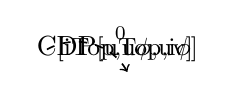
\begin{tikzpicture}[sibling distance=15pt]
			\tikzset{every tree node/.style={align=center,anchor=north}}
			\Tree [.CP \node(C){C\\{\small [iTop,u$ \phi $,uv]}}; [.TP {T$ ^0 $} [.{\ldots} \node(DP){DP\\{\small [uTop,i$ \phi $]}}; [.{\ldots} ] ] ] ]
			\draw[semithick,dashed,->] (DP.west) to [bend left=45] (C.south);
	\end{tikzpicture}
	\end{exe}
\columnbreak
	\begin{exe}
	\ex \label{tree:bk_second} \leavevmode\vadjust{\vspace{-\baselineskip}}\newline
		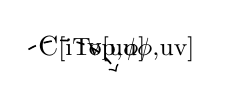
\begin{tikzpicture}[sibling distance=15pt]
			\tikzset{every tree node/.style={align=center,anchor=north}}
			\Tree [.vP \node(v){v\\{\small [u$ \phi $]}}; [.{\ldots} {\ldots} [.CP \node(C){C\\{\small [iTop,u$ \phi $,uv]}}; [.{\ldots} ] ] ] ]
			\draw[semithick,dashed,->] (C.west) to [bend left=45] (v.south);
		\end{tikzpicture}
	\end{exe} 
\end{multicols} \vspace{-0.4cm}
\noindent To establish the second link in the agreement chain, the authors assume that the C head also carries an unvalued feature, namely an unvalued case feature [uv], which allows the C-head to establish an agreement relation with the matrix v, so that v can value its $ \phi $-features (\ref{tree:bk_second}), which then show up as LDA on the matrix verb, following the frequently assumed connection between case assignment and agreement.\footnote{This assumption has frequently been questioned, for example in \citet{Bobaljik2008} and more recently in \citet{Baker_Bobaljik2015} and \cite{Barany2015}.}

Several points of criticism can be raised against this proposal, many of which have already been discussed in \citet{Preminger_Polinsky2015}. From an empirical point of view, there is no obvious explanation for the various blocking effects observed in Tsez. Neither complementizers, nor non-absolutive topics or wh-elements should block the relationship between the C head and the higher \textit{v} since those elements cannot assign case, therefore do not carry a valued v feature and thus cannot intervene in the relation between embedded C and matrix v based on this feature. Second, it seems not straight-forward in this system to derive cross-clausal long distance agreement as can be found in Hinuq (\ref{ex:hinuq_cross-clausal}). While \citet{Polinsky_Potsdam2001} could stipulate successive cyclic LF-movement of the topic DP, \citet{Bjorkman_Zeijlstra2014} would have to assume that each v head that participates in cross-clausal LDA carries its own [uTop] feature to establish an agreement relationship with the next higher C head.

From a theoretical point of view, \citet{Bjorkman_Zeijlstra2014} have to assume that in an extended left periphery in the sense of \citet{Rizzi1997}, it is a language specific property whether the topic head or the focus head hosts the [uv] case feature to account for the fact that in some languages foci can also trigger LDA. However, if it is assumed that this is an idiosyncratic property of a specific head in the left periphery, it becomes impossible to account for the generalization that if foci can trigger LDA in a specific language, this language will have LDA based on topics as well. Additionally, as has been discussed for Uyghur, LDA is sometimes also possible in relative clauses and DP complements. For the approach of \citet{Bjorkman_Zeijlstra2014}, it follows that in these languages, the C head in the periphery of the embedded clause does not carry a [uv]-feature but a [uD]-feature, since, in this case, D is the case assigner, assigning genitive case to the embedded subject. Lastly, turning again to Tsez and other ergative-absolutive languages, linking the assignment of absolutive case to v appears problematic, as absolutive is frequently linked to a higher case assigner since it is usually the unmarked case and shows up, for example, in unaccusatives and passives.

Summing up the discussion, both approaches presented in this section assume some kind of cyclical process that connects matrix verb with embedded agreement goal via an intermediate step in the left periphery. However, both approaches suffer from empirical and theoretical problems that are either linked to the assumption of LF movement as input to later syntactic process or due to the features that are assumed to be involved in the agreement process. In the next section, I will argue for another proposal, that keeps the idea of a cyclic agreement process similar to \citet{Bjorkman_Zeijlstra2014} but does not involve case features.

\section{LDA conditioned by information structure}
\label{ch:4}

I propose to keep the idea of \citet{Bjorkman_Zeijlstra2014} of a cyclic agreement process through the left periphery by capitalizing on the idea that $ \phi $-features can be bundled with information-structural features in the left periphery and that the valuation of the former depends on an agreement process established based on the latter. Concretely, I propose the following structures for the information-structural heads in the left periphery, (\ref{tree:is_top}) for languages like Tsez in which only topics participate in LDA and (\ref{tree:is_foc}) for languages in which this is also possible for foci.
\setlength{\columnsep}{-20pt} %this gives the separation between colums, needs to be defined before multicol is called
\begin{multicols}{2}
	\begin{exe}
	\ex \label{tree:is_top} \leavevmode\vadjust{\vspace{-\baselineskip}}\newline
		\begin{tikzpicture}[sibling distance=15pt]
			\tikzset{every tree node/.style={align=center,anchor=north}}
			\Tree [.Top {Top$^0$\\{\small [iTop:\sqboxEmpty{black}]}} {$\phi$\\{\small [u$\phi$:\sqboxEmpty{black}]}} ]
		\end{tikzpicture}
	\end{exe}
\columnbreak
	\begin{exe}
	\ex \label{tree:is_foc} \leavevmode\vadjust{\vspace{-\baselineskip}}\newline
		\begin{tikzpicture}[sibling distance=15pt]
			\tikzset{every tree node/.style={align=center,anchor=north}}
			\Tree [.Foc {Foc$^0$\\{\small [iFoc:\sqboxEmpty{black}]}} {$\phi$\\{\small [u$\phi$:\sqboxEmpty{black}]}} ]
		\end{tikzpicture}
	\end{exe}
\end{multicols} \vspace{-0.3cm}
\noindent Following \citet{Chomsky2008} and the idea of feature inheritance, I assume that the agreement features that are manifested in T in English and other languages are actually introduced in C, since C is the relevant phase head, and then only inherited by T. The particular type of feature inheritance is, however, a language specific property and \citet{Miyagawa2010,Miyagawa2017} assumes that this is the factor that conditions whether a language is agreement driven or discourse configurational. In the case of the former, for example English, $ \phi $-features are inherited by T and information-structural $ \delta $-features remain in C. In case of the latter, for example Hungarian, it is the reverse, with $ \phi $-features staying in C and $ \delta $ features being inherited by T. In line with \citet{Jimenez-Fernandez2010} and \citet{Miyagawa2017}, I assume that there is a third type, namely languages in which both types of features can remain bundled on the same head giving rise to the structures in (\ref{tree:is_top}) and (\ref{tree:is_foc}).\footnote{The question then arises whether T really inherits the features from C in all cases or whether it is also possible in certain languages that the features are not inherited but copied so that another instance of the feature(-bundle) remains in C.}

Assuming that the left periphery of the embedded clause in LDA contexts contains a head in which $ \phi $- and $ \delta $-features are bundled together provides the intermediate agreement step necessary to connect the higher verb with the lower DP. The derivation for a language like Tsez, in which topicality of the agreement goal is the decisive factor, proceeds as follows. In a first step, represented in (\ref{tree:is_agr1}), the topic head in the left periphery agrees with the embedded topical DP, based on the [uTop]/[iTop] feature pair. At the same time, this allows the $ \phi $-features of the topic head to be valued by the agreed-with DP. In other words, the valuation of the $ \phi $-features depends on an agreement relation established by information-structural features. 
\begin{figure}[!h]
\begin{exe}
\ex \label{tree:is_agr1} \leavevmode\vadjust{\vspace{-\baselineskip}}\newline
	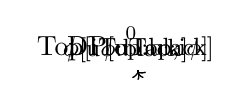
\begin{tikzpicture}[sibling distance=3pt]
		\tikzset{every tree node/.style={align=center,anchor=north}}
		\Tree [.ForceP Force [.TopP [.Top \node(Top){Top\\{\small [iTop:\sqboxEmpty{black}]}}; \node(phi){$\phi$\\{\small [u$\phi$:\sqboxEmpty{black}]}}; ] [.{\ldots} {\ldots} [.TP {T$ ^0 $} [.{\ldots} \node(DP){DP\\{\small [uTop,i$ \phi $]}}; [.{\ldots} ] ] ] ] ] ]
		\draw[semithick,dashed,->] (Top.south) to [bend right=45] (DP.south);
		\draw[semithick,dashed,->] (phi.south) to [bend right=45] (DP.south);
	\end{tikzpicture}
\end{exe}
\end{figure}
In a second step, matrix v with its own set of unvalued $ \phi $-features probes in its c-command domain and agrees with the $ \phi $-features that are now hosted by the topic head in the periphery of the embedded clause.\footnote{In contrast to \citet{Bjorkman_Zeijlstra2014}, I only link $ \phi $-feature agreement to v and not to absolutive case.} Under the assumption that the verb in the matrix clause moves at least as high as v, these $ \phi $-features then end up being spelled out on the matrix verb.
\begin{figure}[!h]
\begin{exe}
\ex \label{tree:is_agr2} \leavevmode\vadjust{\vspace{-\baselineskip}}\newline
	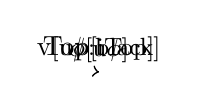
\begin{tikzpicture}[sibling distance=3pt]
		\tikzset{every tree node/.style={align=center,anchor=north}}
		\Tree [.vP \node(v){v\\{\small [u$\phi$:\sqboxEmpty{black}]}}; [.{\ldots} {\ldots} [.TopP [.Top \node(Top){Top\\{\small [iTop]}}; \node(phi){$\phi$\\{\small [u$\phi$]}}; ] {\ldots}  ] ] ] 
		\draw[semithick,dashed,->] (v.south) to [bend right=80] (phi.south);
	\end{tikzpicture}\vspace{-1cm}
\end{exe} \vspace{-0.4cm}
\end{figure}
In this proposal, most of the properties of LDA that have been discussed above can easily be accounted for. First, the blocking effect of non-absolutive topics is simply due to the fact that only absolutive arguments can participate in $ \phi $-feature agreement. Thus, even though an agreement relation between topic head and embedded non-absolutive topic can be established, the $ \phi $-features on the topic head remain unvalued, leading to the spell-out of the default agreement on matrix v. Similarly, under the assumption that $ \phi $-features are also present on complementizers, those features provide a closer agreement goal for v than the $ \phi $-features of the embedded topic. However, since the complementizer does not carry absolutive case, v cannot agree with it, leading again to the spell out of the default feature value. Appealing to locality can also account for the observation that absolutive wh-elements can lead to LDA. LDA is possible when the agreement goal manages to get high enough in the periphery of the embedded clause. Since wh-elements are usually connected to the left periphery by either movement or agreement, their participation in LDA is expected, as long as they carry absolutive case.\footnote{This property of LDA has been exploited by \citet{Heck_Cuartero2012} in their analysis of relative clauses as involving a particular form of LDA.}

Turning to properties of LDA in languages other than Tsez, the generalization that if foci can participate in LDA in a particular language, topics can participate as well follows directly from the dependence on information structure and the fine structure of the left periphery as assumed by \citet{Rizzi1997}, as exemplified in (\ref{ex:left-periphery2}).
\begin{exe} \label{ex:left-periphery2}
	\ex {[}\sub{ForceP} Force [\sub{TopP*} Top [\sub{FocP} Foc [\sub{TopP*} Top [\sub{FinP} Fin [ {\ldots} ] ] ] ] ] ] 
\end{exe}
It is generally assumed that, in a left periphery hosting information-structural projections, the focus phrase is sandwiched between two topic phrases. Thus, the presence of a focus phrase always entails the presence of a higher topic phrase. Consequently, if a focus phrase counts a sufficiently local to the higher matrix v, the  topic phrase dominating the focus phrase necessarily is local enough as well so that if foci can participate in LDA, so will topics.

LDA across more than one CP boundary is also expected in this approach. Nothing prevents intermediate topic heads from probing for a topicalized element in their c-command domain. For these heads, the initial topicalized DP in the lowest clause is not accessible since it is not local enough, i.e. separated by at least one CP boundary. However, they can agree with the topic head in the left periphery of the next lower clause. Since this topic head also hosts $ \phi $-features which have been valued by the topicalized DP in the lowest clause, the intermediate topic head can also value its $ \phi $-features, in effect transmitting the $ \phi $-features of the topicalized DP up until v in the highest clause.\footnote{I ignore the vP here. If vP is indeed a phase, then its periphery might host information structural projections as well which then participate in successive-cyclic agreement.}

Note that this approach predicts that it is impossible for LDA to skip an intermediate clause. Thus, in a structure with three clauses, it is impossible for the verb in the highest clause to show LDA with the topic of the lowest clause if the verb in the intermediate clause does not show LDA as well. Since cross clausal LDA is successive cyclic as well, all intermediate topic heads need to participate in it, otherwise the $ \phi $-feature of the topic in the lowest clause cannot be accessed by higher verbs. As has been discussed above, this prediction is borne out in Hinuq (\ref{ex:hinuq_cross-clausal}) and cross-clausal LDA cannot skip an intermediate clause.

Lastly, the approach presented in this section is independent of the element in the matrix clause that establishes the actual agreement relation into the embedded clause. In the Nakh-Dagestanian and Algonquian languages, this element appears to be v, whereas in Uyghur it is a D head in the higher clause.

In sum, the present approach appears to be advantageous over the approaches of \citet{Polinsky_Potsdam2001} as well as \citet{Bjorkman_Zeijlstra2014} discussed above in that it easily derives the cross-linguistic properties of long distance agreement without any stipulations that cannot independently be motivated.

\section{Conclusion}
\label{ch:5}

In this paper, I have presented a successive cyclic approach to long distance agreement that is based on the bundling of $ \phi $- and $ \delta $-features on heads in the left periphery of the embedded clause. Starting from an extensive typological discussion, I have shown that LDA can be found in various unrelated language families, namely in Nakh-Dagestanian, Algonquian and Altaic languages, albeit with slightly different properties. A generalization emerged from this discussion, namely that if a language permits LDA based on embedded foci it will also allow LDA based on embedded topics.

In the second part, after discussing previous analyses of LDA, I presented an approach that derives long distance agreement via successive cyclic agreement through the periphery of the embedded clause, thus analyzing LDA in accordance with the PIC, and similar to successive cyclic wh-movement. The nature of the intermediate head in the left periphery was then the main ingredient of the analysis in which I assumed a particular notion of feature inheritance. In addition to either transmitting $ \phi $- or $ \delta $-features from C to T, both can remain in C bundled together on one head. The valuation of one part of the feature bundle then depended on an agreement relation established based on the other part. More concretely, the head in the left periphery established an agreement relation with the relevant DP based on $ \delta $-features which allowed the $ \phi $-features of the left-peripheral head to be valued as well. For the second step in this successive cyclic agreement, the $ \phi $-features on this head then served as agreement goal for a higher probing head in the matrix clause, v or D. These assumptions, combined with a standard analysis of the left periphery, were then able to derive the cross-linguistic properties of LDA.

If this analysis is on the right track, more instances of information-structurally influenced $ \phi $-feature agreement are to be expected in various languages, see for example \textcitetv{chapters/08-dalessandro} for topic agreement in Ripano, \citet{Dalrymple_Nikolaeva2011} for the connection between objects and information structure more generally, and van der Wal (2015, 2019) for an overview of object marking in Bantu. \nocite{Van_der_Wal2015,chapters/07-van-der-wal} %CHECK if this works

\section*{Abbreviations}
Roman numerals refer to noun classes, Arabic numerals followed by \textsc{sg/pl} refer to person.
\begin{table}
	\begin{tabular}{llllll} 
	\textsc{abs} 	&	 absolutive 	&	\textsc{f} 	&	  feminine 	&	  \textsc{perf} 	&	   perfect 	\\
\textsc{abst} 	&	  abstract suffix 	&	  \textsc{foc} 	&	  focus	&	  \textsc{pfv} 	&	  perfective 	\\
\textsc{acc} 	&	  accusative 	&	  \textsc{fut} 	&	  future	&	  \textsc{poss}  	&	 possessive 	\\
\textsc{ai} 	&	  animate intrans. 	&	  \textsc{gen} 	&	  genitive  	&	  \textsc{pret} 	&	  preterite 	\\
\textsc{an} 	&	  animate 	&	  \textsc{hab} 	&	  habitual 	&	  \textsc{prox}  	&	 proximal 	\\
\textsc{aor} 	&	  aorist 	&	  \textsc{impf} 	&	  imperfective	&	  \textsc{prs} 	&	  present 	\\
\textsc{appl} 	&	  applicative 	&	  \textsc{inan} 	&	  inanimate	&	  \textsc{pst} 	&	  past 	\\
\textsc{aug} 	&	  augmentative 	&	  \textsc{inv} 	&	  inverse	&	  \textsc{ptcp} 	&	  participle 	\\
\textsc{c}	&	complementizer	&	  \textsc{lat} 	&	  lative 	&	  \textsc{purp}  	&	 purposive 	\\
\textsc{caus} 	&	  causative 	&	  \textsc{loc} 	&	  locative	&	\textsc{q}	&	question particle	\\
\textsc{conj} 	&	  conjunct 	&	  \textsc{n} 	&	  neuter 	&	  \textsc{quot} 	&	  quotative 	\\
\textsc{cvb} 	&	  converb 	&	  \textsc{neg} 	&	  negation 	&	\textsc{recp}	&	reciprocal	\\
\textsc{dat} 	&	  dative 	&	  \textsc{nom} 	&	  nominative 	&	  \textsc{res} 	&	  resultative 	\\
\textsc{dem} 	&	  demonstrative 	&	  \textsc{obl} 	&	  oblique	&	  \textsc{sm} 	&	  subject marker 	\\
\textsc{dir} 	&	  directional 	&	  \textsc{obv} 	&	  obviative	&	  \textsc{ta} 	&	  trans. animate 	\\
\textsc{erg} 	&	  ergative 	&	  \textsc{om} 	&	  object marker	&	  \textsc{ti} 	&	  trans. inanimate 	\\
\textsc{emph} 	&	  emphatic particle 	&	  \textsc{pl} 	&	  plural	&	  \textsc{top} 	&	  topic 	\\
\textsc{evid} 	&	  evidential 	&	  \textsc{part} 	&	  participle agr. 	&	  \textsc{uwpst} 	&	  unwitnessed pst	
	\end{tabular}		
\end{table}


\section*{Acknowledgements}

The topic was (in part) presented at the IGG 2017, at Goethe University Frankfurt and the EGG 2016, and I thank the audiences for their comments and suggestions. The research has also benefited greatly from discussions with Katharina Hartmann, Peter Smith, Jennifer Tan, Hedde Zeijlstra and Jonathan Bobaljik, as well as the comments and suggestions of two reviewers. All shortcomings remain my own.

\printbibliography[heading=subbibliography,notkeyword=this]

\end{document}
